\section{Sviluppo}

\subsection{Ghost area}

Entrambe le soluzioni proposte si avvalgono dell'utilizzo di una ghost area
inizializzata a zero (e mai più modificata).

Ciò permette di ridurre notevolmente l'impatto sulle prestazioni
dell'operazione di propagazione, poiché, avendo una nuova regione di celle
intorno al dominio, non sarà più necessario controllare che le celle adiacenti a
quella presa in esame siano ai bordi del dominio stesso.
Il valore delle ghost cell (zero), inoltre, non influirà sui risultati delle
operazioni dell'algoritmo.

In figura \ref{fig:ghostarea}(\cite{marzollaghost}) è possibile osservare il comportamento appena
descritto.

\begin{figure}[!ht]
  \centering
  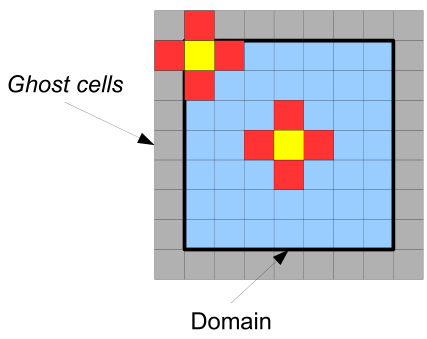
\includegraphics[scale=0.3]{./ghost-area.png}
  \caption{Rappresentazione della ghost area (celle
  grigie).}\label{fig:ghostarea}
\end{figure}

\subsection{Accesso in memoria al dominio}

È stato inizialmente ipotizzato l'accesso alla matrice considerandola come un
array, in accordo con la rappresentazione in memoria delle matrici fornita dal
linguaggio C.
Ciò avrebbe permesso di scorrere in modo sequenziale la matrice stessa,
risparmiando le chiamate alla funzione \texttt{IDX}.

Ad esempio, l'operazione di incremento di energia sarebbe stata implementata nel
seguente modo:
\begin{minted}{c}
for (int i = 0; i < n; i++) {
    grid[i] += delta;
}
\end{minted}

Tuttavia, l'introduzione della \textit{ghost area} ha reso preferibile (in
termini di gestione dell'accesso alla memoria) l'utilizzo della funzione
\texttt{IDX}, che contribuisce inoltre ad una buona comprensione e leggibilità
del codice sorgente.

\subsection{Versione OpenMP}

In figura \ref{fig:simulation1} è possibile osservare il risultato della
simulazione in termini di energia media delle celle e numero di celle che hanno
superato il valore soglia, misurate ad ogni passo di esecuzione.

\begin{figure}[!ht]
  \centering
  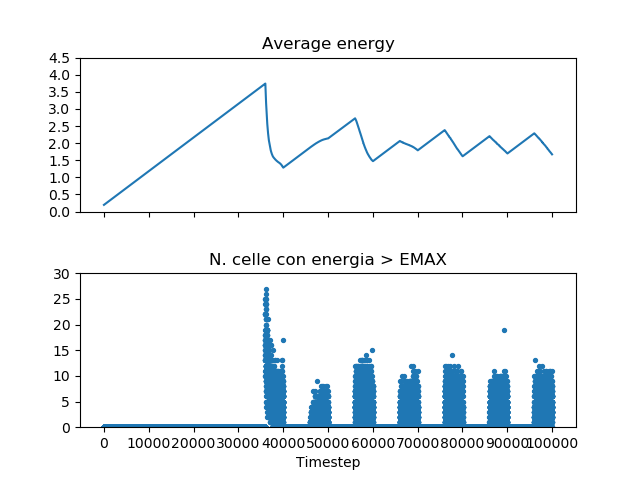
\includegraphics[scale=0.55]{./graphs/omp-earthquake.png}
  \caption{Risultato della simulazione.}\label{fig:simulation1}
\end{figure}

\subsubsection{Modifiche alla versione seriale}

\paragraph{setup}L'inizializzazione della ghost area a zero non è stata
parallelizzata poiché i test effettuati e mostrati nella tabella
\ref{tab:parallelghostarea} hanno evidenziato un degradamento, seppur minimo,
delle prestazioni.

\begin{table}[ht]
\centering
\begin{tabular}{rccc}
\cmidrule[\heavyrulewidth]{2-4}
 & Lato dominio & Numero passi & T\textsubscript{setup} (\textit{s})\\
 \cmidrule[\lightrulewidth]{2-4}
 seriale & \multirow{2}{*}{512} & \multirow{2}{*}{1000} & 0.00337177\\
 parallelizzato &&& 0.00454419\\
\cmidrule[\heavyrulewidth]{2-4}
\end{tabular}
\caption{\label{tab:parallelghostarea}Confronto dei tempi di esecuzione per la
funzione \texttt{setup} nella versione seriale e nella versione parallelizzata.}
\end{table}

Tale comportamento può essere dovuto ad un ulteriore carico di lavoro assegnato
allo scheduler per un'attività che mal si presta (soprattutto per l'accesso ai
lati sinistro e destro del dominio a causa dell'accesso in memoria) ad essere
parallelizzata.

\paragraph{altre operazioni}
Tutte le principali operazioni (incremento, conteggio, propagazione e calcolo
energia media) contengono dei cicli \texttt{for} che sono stati parallelizzati
utilizzando la direttiva OpenMP \texttt{omp parallel for}.  In tale modo
l'intero carico di lavoro del ciclo a cui è stato applicato il costrutto viene
suddiviso tra i thread che concorrono all'esecuzione del programma, realizzando
la vera e propria parallelizzazione.

Nelle operazioni di conteggio e di calcolo dell'energia media è stata inoltre
introdotta la clausola di riduzione con l'operatore somma, per poter
parallelizzare anche le operazioni di somma all'interno delle direttive OpenMP\@.

\subsubsection{Ulteriori ottimizzazioni}

\paragraph{collapse}

È stato valutato l'utilizzo della clausola \texttt{collapse(2)} sui cicli
\texttt{for} innestati per collassare le due iterazioni in una, allargando lo
spazio di iterazione come da specifiche\cite{openmp2018reference}.

Tale clausola ha tuttavia causato un degrado delle prestazioni (si veda la
tabella \ref{tab:collapse}) e pertanto non è stata implementata nella soluzione proposta.

\begin{table}[ht]
\begin{tabularx}{\linewidth}{rXXXXX}
\cmidrule[\heavyrulewidth]{2-6}
& Lato dom. & \# passi & $\overline{T}$\textsubscript{3-run}(\textit{s})
& cache-references (M/sec) & cache-misses (\%)*\\
\cmidrule[\lightrulewidth]{2-6}
senza \texttt{collapse(2)} & \multirow{2}{*}{256} & \multirow{2}{*}{100000} &
   13.33183 & 0.770 & 0.390\\
\cmidrule{4-6}
   con \texttt{collapse(2)} &&& 19.18336 & 0.560 & 0.402\\
\cmidrule[\heavyrulewidth]{2-6}
\end{tabularx}
\caption{\label{tab:collapse}Dati raccolti sull'esecuzione della simulazione con
e senza la direttiva \texttt{collapse(2)}.}
\end{table}

*: of all cache refs.

Dai dati presenti in tabella è possibile osservare che, al contrario di come ci
si aspetterebbe, nonostante la clausola \texttt{collapse} modifichi i
\textit{chunk} di memoria a cui si accede, ciò non comporta un degradamento
significativo delle prestazioni nell'accesso alla memoria cache.

Di conseguenza si ipotizza che l'incremento delle tempistiche di esecuzione
possa essere legato ad una cattiva gestione da parte dello scheduler
nell'organizzare il lavoro dei thread.

\paragraph{schedule}

È stata inoltre valutata l'adozione della clausola \texttt{schedule},
utilizzando il parametro \texttt{type} nelle sue varianti \texttt{static},
\texttt{dynamic} e \texttt{guided}.
%Si rimanda alle specifiche \cite{openmp2018reference} per ulteriori dettagli su
%tale operatore.

Le prove effettuate hanno mostrato un significativo aumento delle prestazioni
impostando uno scheduling statico con blocchi di dimensione 8.

La tabella \ref{tab:schedule} mostra la differenza di tempistiche medie (su 3
esecuzioni) tra la versione in cui la clausola \texttt{schedule} non è
specificata e quella in cui viene usata con parametri \texttt{static, 8}.

\begin{table}[ht]
\centering
\begin{tabularx}{400pt}{XXXX}
\toprule
Lato dom. & \# passi & $\overline{T}$\textsubscript{3-run}(\textit{s})&
$\overline{T}$\textsubscript{3-run}(\textit{s}) con \texttt{schedule(static,8)}\\
\midrule
 256 & \multirow{3}{*}{100000} & 12.9581 & 10.3148 \\
 512 && 50.4409 & 40.5048 \\
 1024 && 250.4084 & 177.2195 \\
\bottomrule
\end{tabularx}
\caption{\label{tab:schedule}Comparazione delle tempistiche di esecuzione
applicando uno scheduling statico.}
\end{table}

Tale clausola ha quindi permesso una importante riduzione delle tempistiche,
compresa tra il 20 e il 30\% in meno rispetto alla precedente versione già
parallelizzata.

Altri tipi di scheduling o diverse dimensioni dei \textit{chunk} hanno
pareggiato o addirittura peggiorato le precedenti tempistiche.

%Poiché le quattro operazioni fondamentali necessitano di essere eseguite in uno
%specifico ordine, non è stato possibile valutare altre ottimizzazioni o API
%di OpenMP per ottimizzare l'esecuzione.
%La principale è \texttt{parallel for}.

\subsection{Versione CUDA}

Il dominio è stato partizionato, come da suggerimenti, in blocchi 2D organizzati
a loro volta in griglie 2D.

Per le operazioni effettuate nelle funzioni \texttt{count\_cells} e
\texttt{average\_energy} il dominio è stato invece partizionato in blocchi
monodimensionali, in accordo con la rappresentazione matriciale nel linguaggio
di programmazione C.

A tal proposito, per le sopracitate operazioni, è stata opportunamente
implementata l'operazione di riduzione mediante operatore somma.

In un primo momento, per semplicità, si è proceduto con la realizzazione della
soluzione senza l'utilizzo della memoria condivisa del Device.
